\section{Giới thiệu Grafana}
Grafana là một nền tảng mã nguồn mở hỗ trợ mạnh mẽ cho việc theo dõi và đánh giá các số liệu thu thập được. Vì vậy, Grafana có thể được ứng dụng rộng rãi trong nhiều lĩnh vực khác nhau chứ không chỉ riêng công nghệ thông tin. Bất kì lĩnh vực nào có thể thu thập được dữ liệu theo dòng thời gian đều có thể tối ưu trực quan hóa trên Grafana.
Đối với việc quản trị vận hành phần mềm, Grafana là công cụ hỗ trợ mạnh mẽ việc trực quan hóa các chỉ số (ví dụ như cpu, ram, dish, network, iops, session,…) và nhật ký hoạt động được thu thập từ ứng dụng. Nó có thể kết nối được với nhiều nguồn dữ liệu khác nhau như Prometheus, InfluxDB, ElasticSearch và các công cụ cơ sở dữ liệu quan hệ truyền thống. Nhờ vậy mà ta có thể truy vấn, trực quan hóa, cảnh báo và tìm hiểu dữ liệu bất kể chúng được lưu trữ ở đâu, từ đó tạo ra những hệ thống giám sát sinh động, linh hoạt, dễ dàng nắm bắt thông tin và kiểm soát trạng thái của ứng dụng. 

Cùng với sự phát triển của doanh nghiệp, dữ liệu cũng ngày càng lớn hơn, và ta cần phải kết nối chúng với nhau để nắm được thông tin một cách toàn diện. Khi đó, Grafana sẽ là một chất kết dính mãnh mẽ cho phép kết nối dữ liệu từ nhiều nguồn khác nhau để nhanh chóng tạo nên một bức tranh toàn cảnh tại mọi thời điểm cần thiết. Grafana có rất nhiều điểm nổi bật, trong đó không thể không thể kể đến một số đặc điểm quan trọng sau đây:
\begin{itemize}
    \item \textit{Hợp nhất dữ liệu, thay vì hợp nhất cơ sở dữ liệu (database)}:Grafana không yêu cầu bạn phải nhập dữ liệu vào một cơ sở dữ liệu cụ thể. Thay vào đó, Grafana hợp nhất các dữ liệu mà bạn đang có, bất kể chúng đang được lưu trữ ở đâu, trên cùng một hệ thống hay nhiều hệ thống khác nhau.
    \item \textit{Mọi người đều có thể tiếp cận được tới dữ liệu}: Grafana được xây dựng dựa trên nguyên tắc là mọi người đều có thể truy cập vào dữ liệu trong tổ chức, chứ không chỉ riêng người vận hành ứng dụng. Bằng cách dân chủ hóa quyền truy cập dữ liệu, Grafana giúp thúc đẩy văn hóa chia sẻ dữ liệu và thúc đẩy dữ liệu được sử dụng bởi những người thực sự cần nó, phá vỡ những rào cản và trao quyền cho các đội nhóm. Tất nhiên, trong trường hợp bạn muốn giới hạn quyền tiếp cận dữ liệu đối với từng người dùng, Grafana phiên bản Cloud và Enterprise cũng hỗ trợ cho phép thực hiện các chế độ bảo mật thông tin như vậy.
    \item \textit{Dashboard mà mọi người đều có thể sử dụng được}: Với Grafana, bạn không chỉ nhận được các thông tin giá trị từ dữ liệu được thu thập từ nhiều nguồn, mà còn có thể chia sẻ các dashboard với các thành viên khác trong đội nhóm, cho phép mọi người có thể cùng nhau khám phá, tìm hiểu dữ liệu.
    \item \textit{Linh hoạt và đa năng}: Grafana có thể chuyển đổi bất kì dữ liệu nào của bạn thành nhưng dashboard có tính linh hoạt và đa năng cao. Không giống như các công cụ khác, Grafana cho phép bạn xây dựng các dashboard một cách cụ thể theo mục đích mong muốn của bạn. Với khả năng truy vấn và chuyển hóa dữ liệu tiên tiến, bạn có thể thiết kế các panels may đo theo hướng thuận tiện nhất cho mình.
\end{itemize}

\begin{figure}[H] % places figure environment here   
    \centering % Centers Graphic
    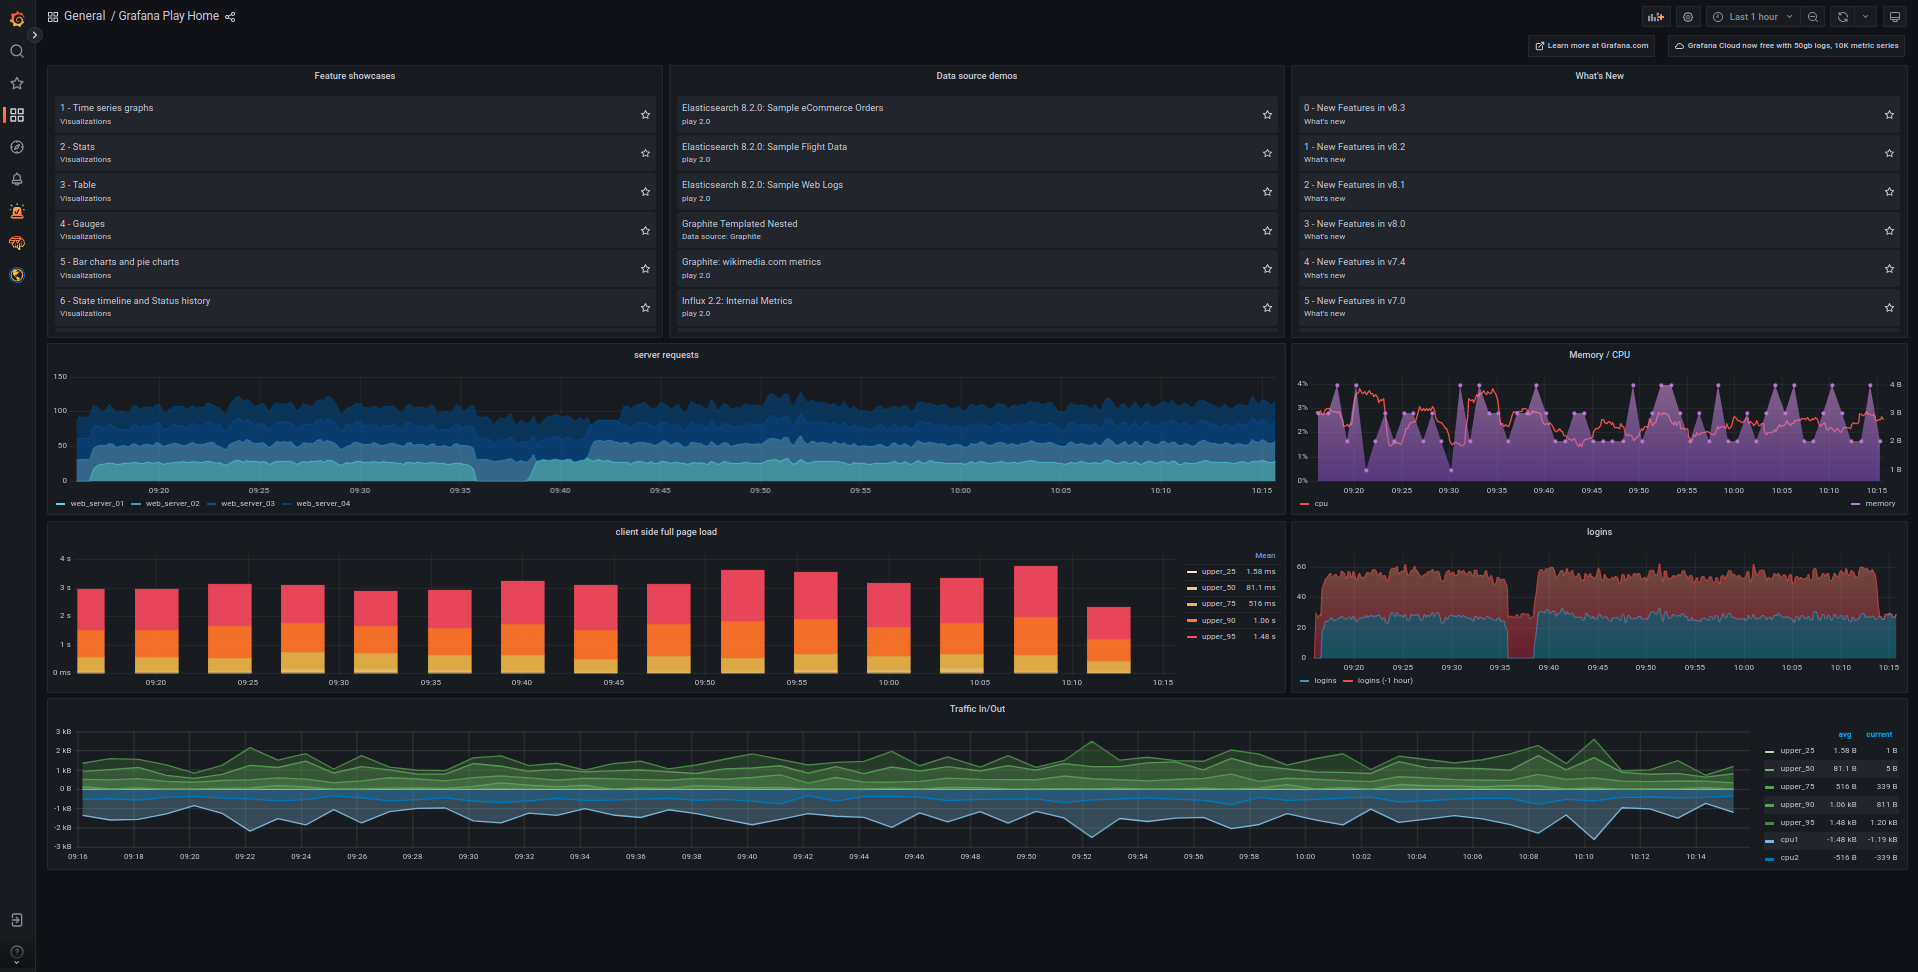
\includegraphics[width=1\textwidth]{figures/fig_01.png} 
    \caption{Một dashboard demo trên trang chủ của Grafana} % Creates caption underneath graph
    \label{fig:fig_01}
\end{figure}
Hình 2.1 thể hiện ví dụ về một dashboard được xây dựng với Grafana. Biểu đồ trên cùng bên trái thể hiện lượng requests tới một website nào đó trong khoảng thời gian một giờ gần nhất. Không chỉ thể hiện tổng lượng request, ta còn có thể quan sát thấy thông lượng tới từng node từ web\_server\_01 đến web\_server\_04 thông qua lớp phủ màu. Ngoài ra khi giữ chuột vào một thời điểm nhất định, biểu đồ cũng cho biết số lượng request cụ thể vào từng node vào thời điểm đó. Biểu đồ trên cùng bên phải thể hiện tài nguyên Memory và CPU được sử dụng của ứng dụng. Các biểu đồ tiếp theo lần lượt đưa ra các chỉ số khác cần theo dõi của ứng dụng.

Grafana có thể ứng dụng với các dashboard trong nhiều lĩnh vực khác nhau, với đa dạng các mục đích. Dưới đây là một số ví dụ minh họa khác về dashboard được xây dựng với Grafana.
\begin{figure}[H] % places figure environment here   
    \centering % Centers Graphic
    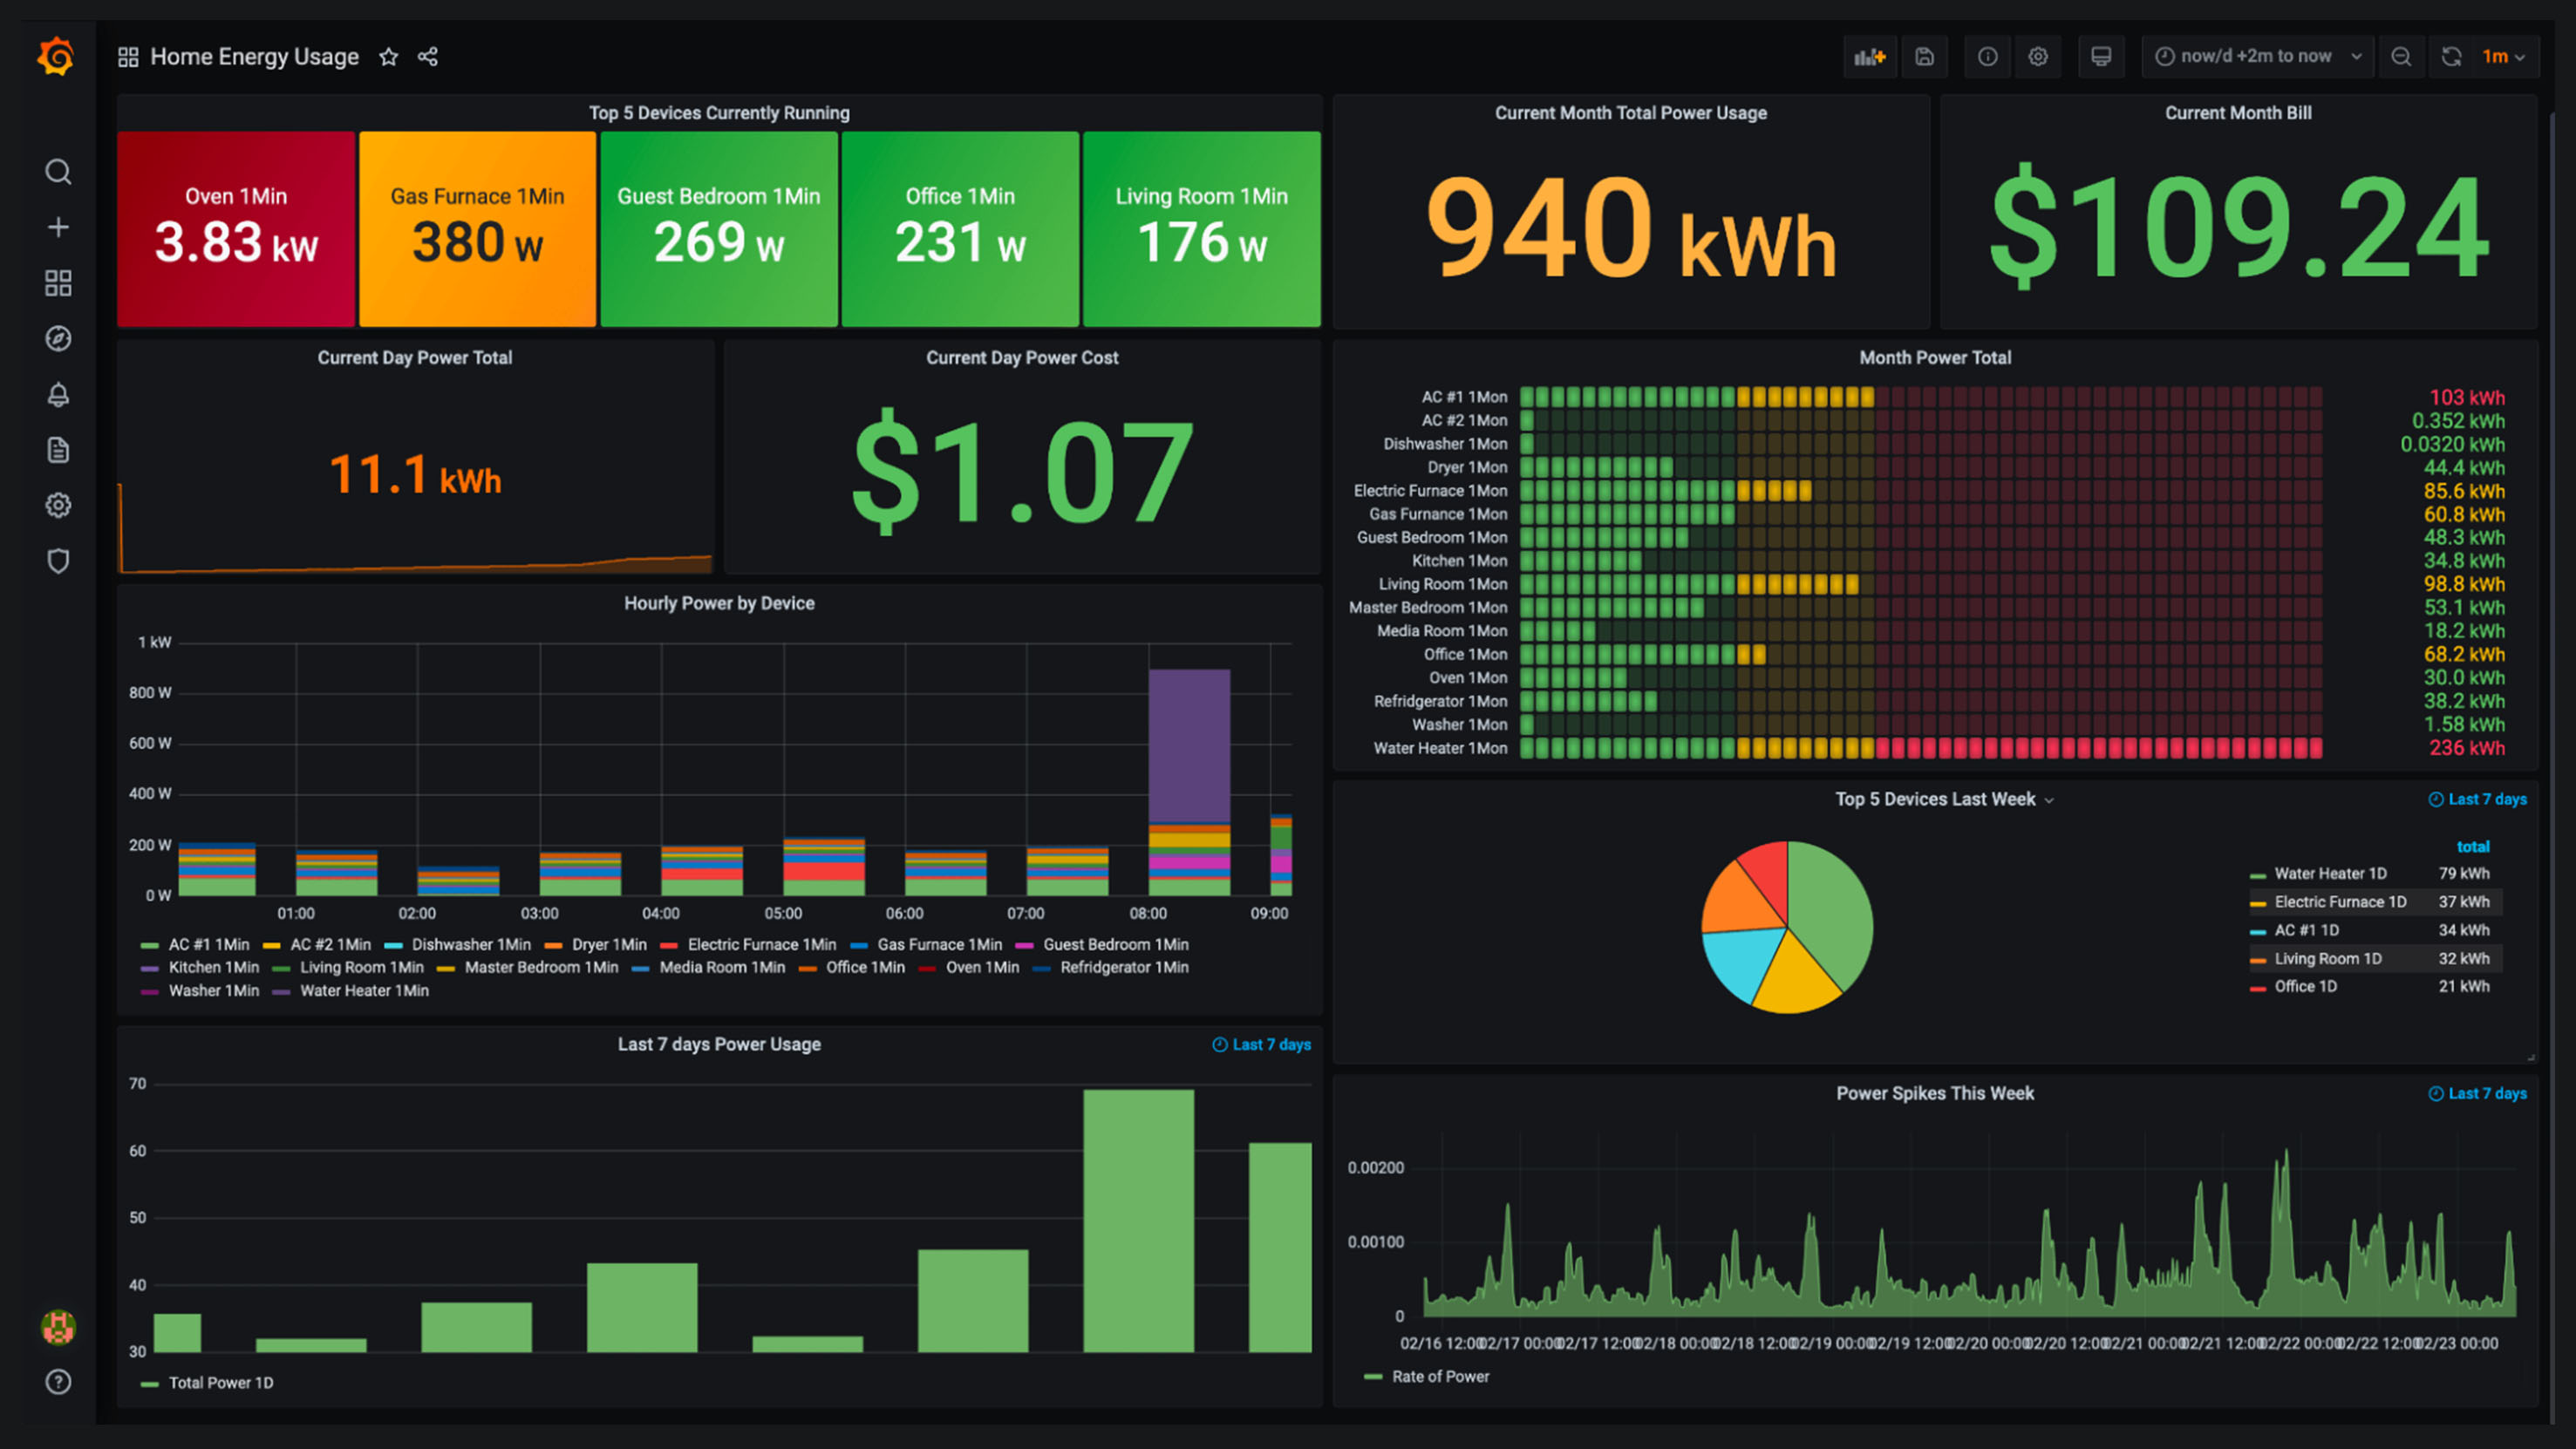
\includegraphics[width=1\textwidth]{figures/Grafana8_HomeEnergy.jpg} 
    \caption{Dashboard đo lường năng lượng tiêu thụ trong hộ gia đình} % Creates caption underneath graph
    \label{fig:fig_01}
\end{figure}
\begin{figure}[H] % places figure environment here   
    \centering % Centers Graphic
    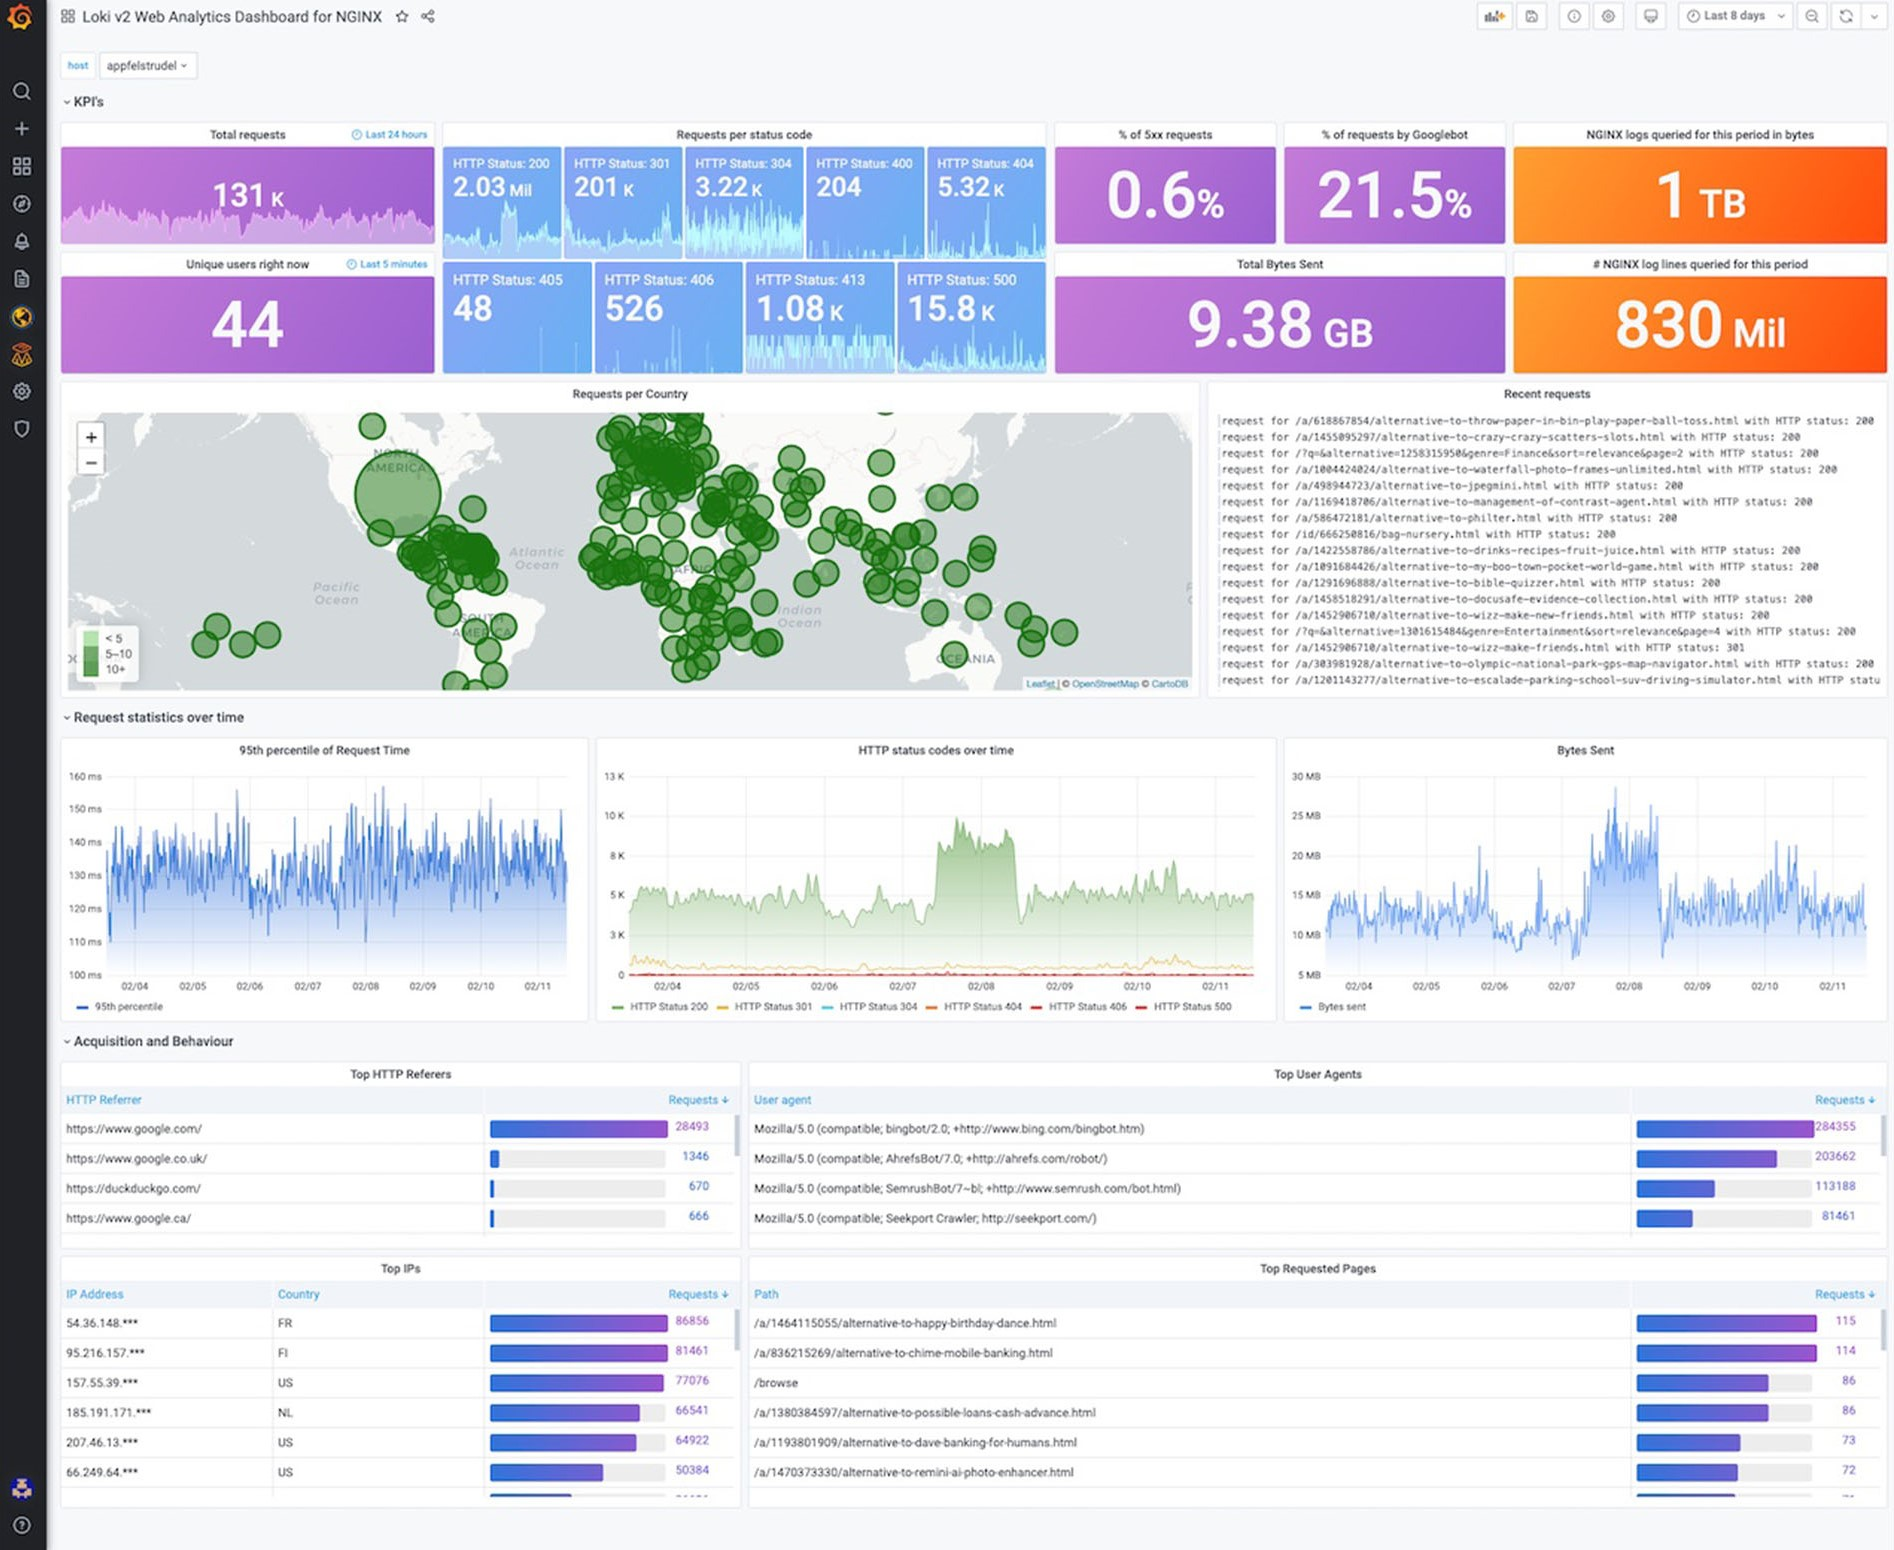
\includegraphics[width=1\textwidth]{figures/Grafana8_WebsitePerformance.jpg} 
    \caption{Dashboard theo dõi hiệu quả của một website} % Creates caption underneath graph
    \label{fig:fig_01}
\end{figure}
\begin{figure}[H] % places figure environment here   
    \centering % Centers Graphic
    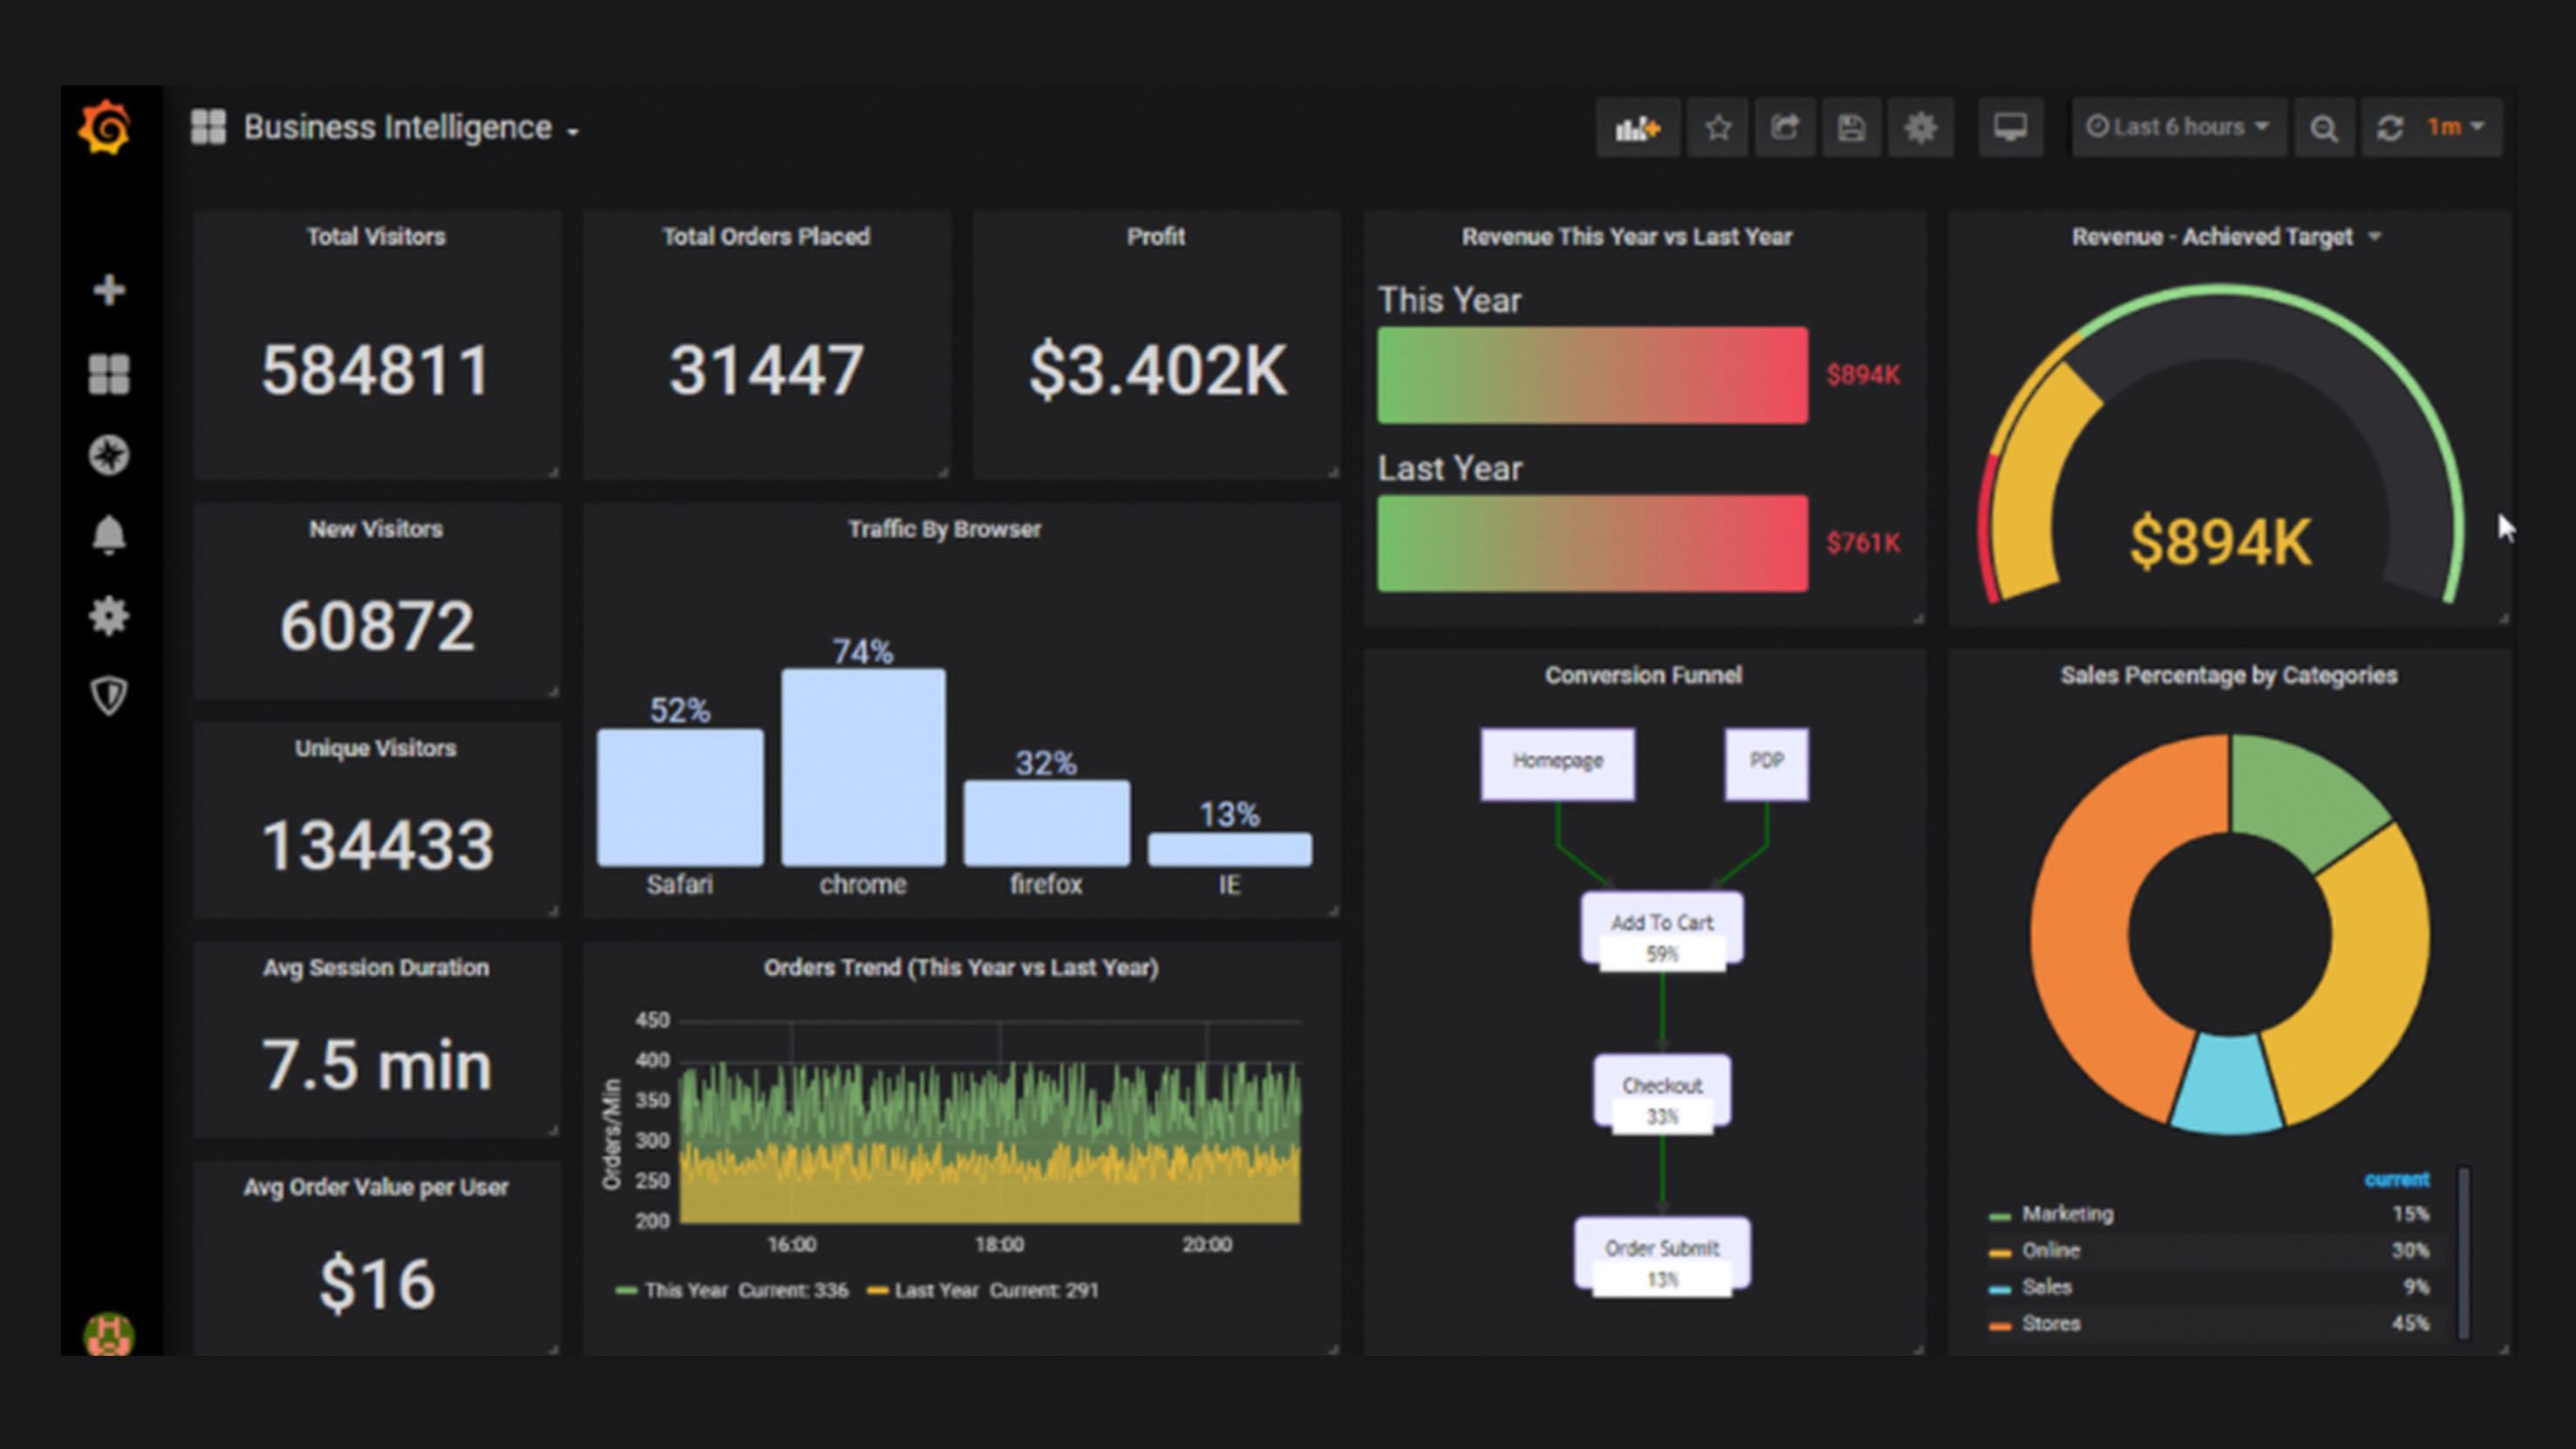
\includegraphics[width=1\textwidth]{figures/Grafana8_Revenue.jpg} 
    \caption{Dashboard theo dõi doanh thu kinh doanh} % Creates caption underneath graph
    \label{fig:fig_01}
\end{figure}
\begin{figure}[H] % places figure environment here   
    \centering % Centers Graphic
    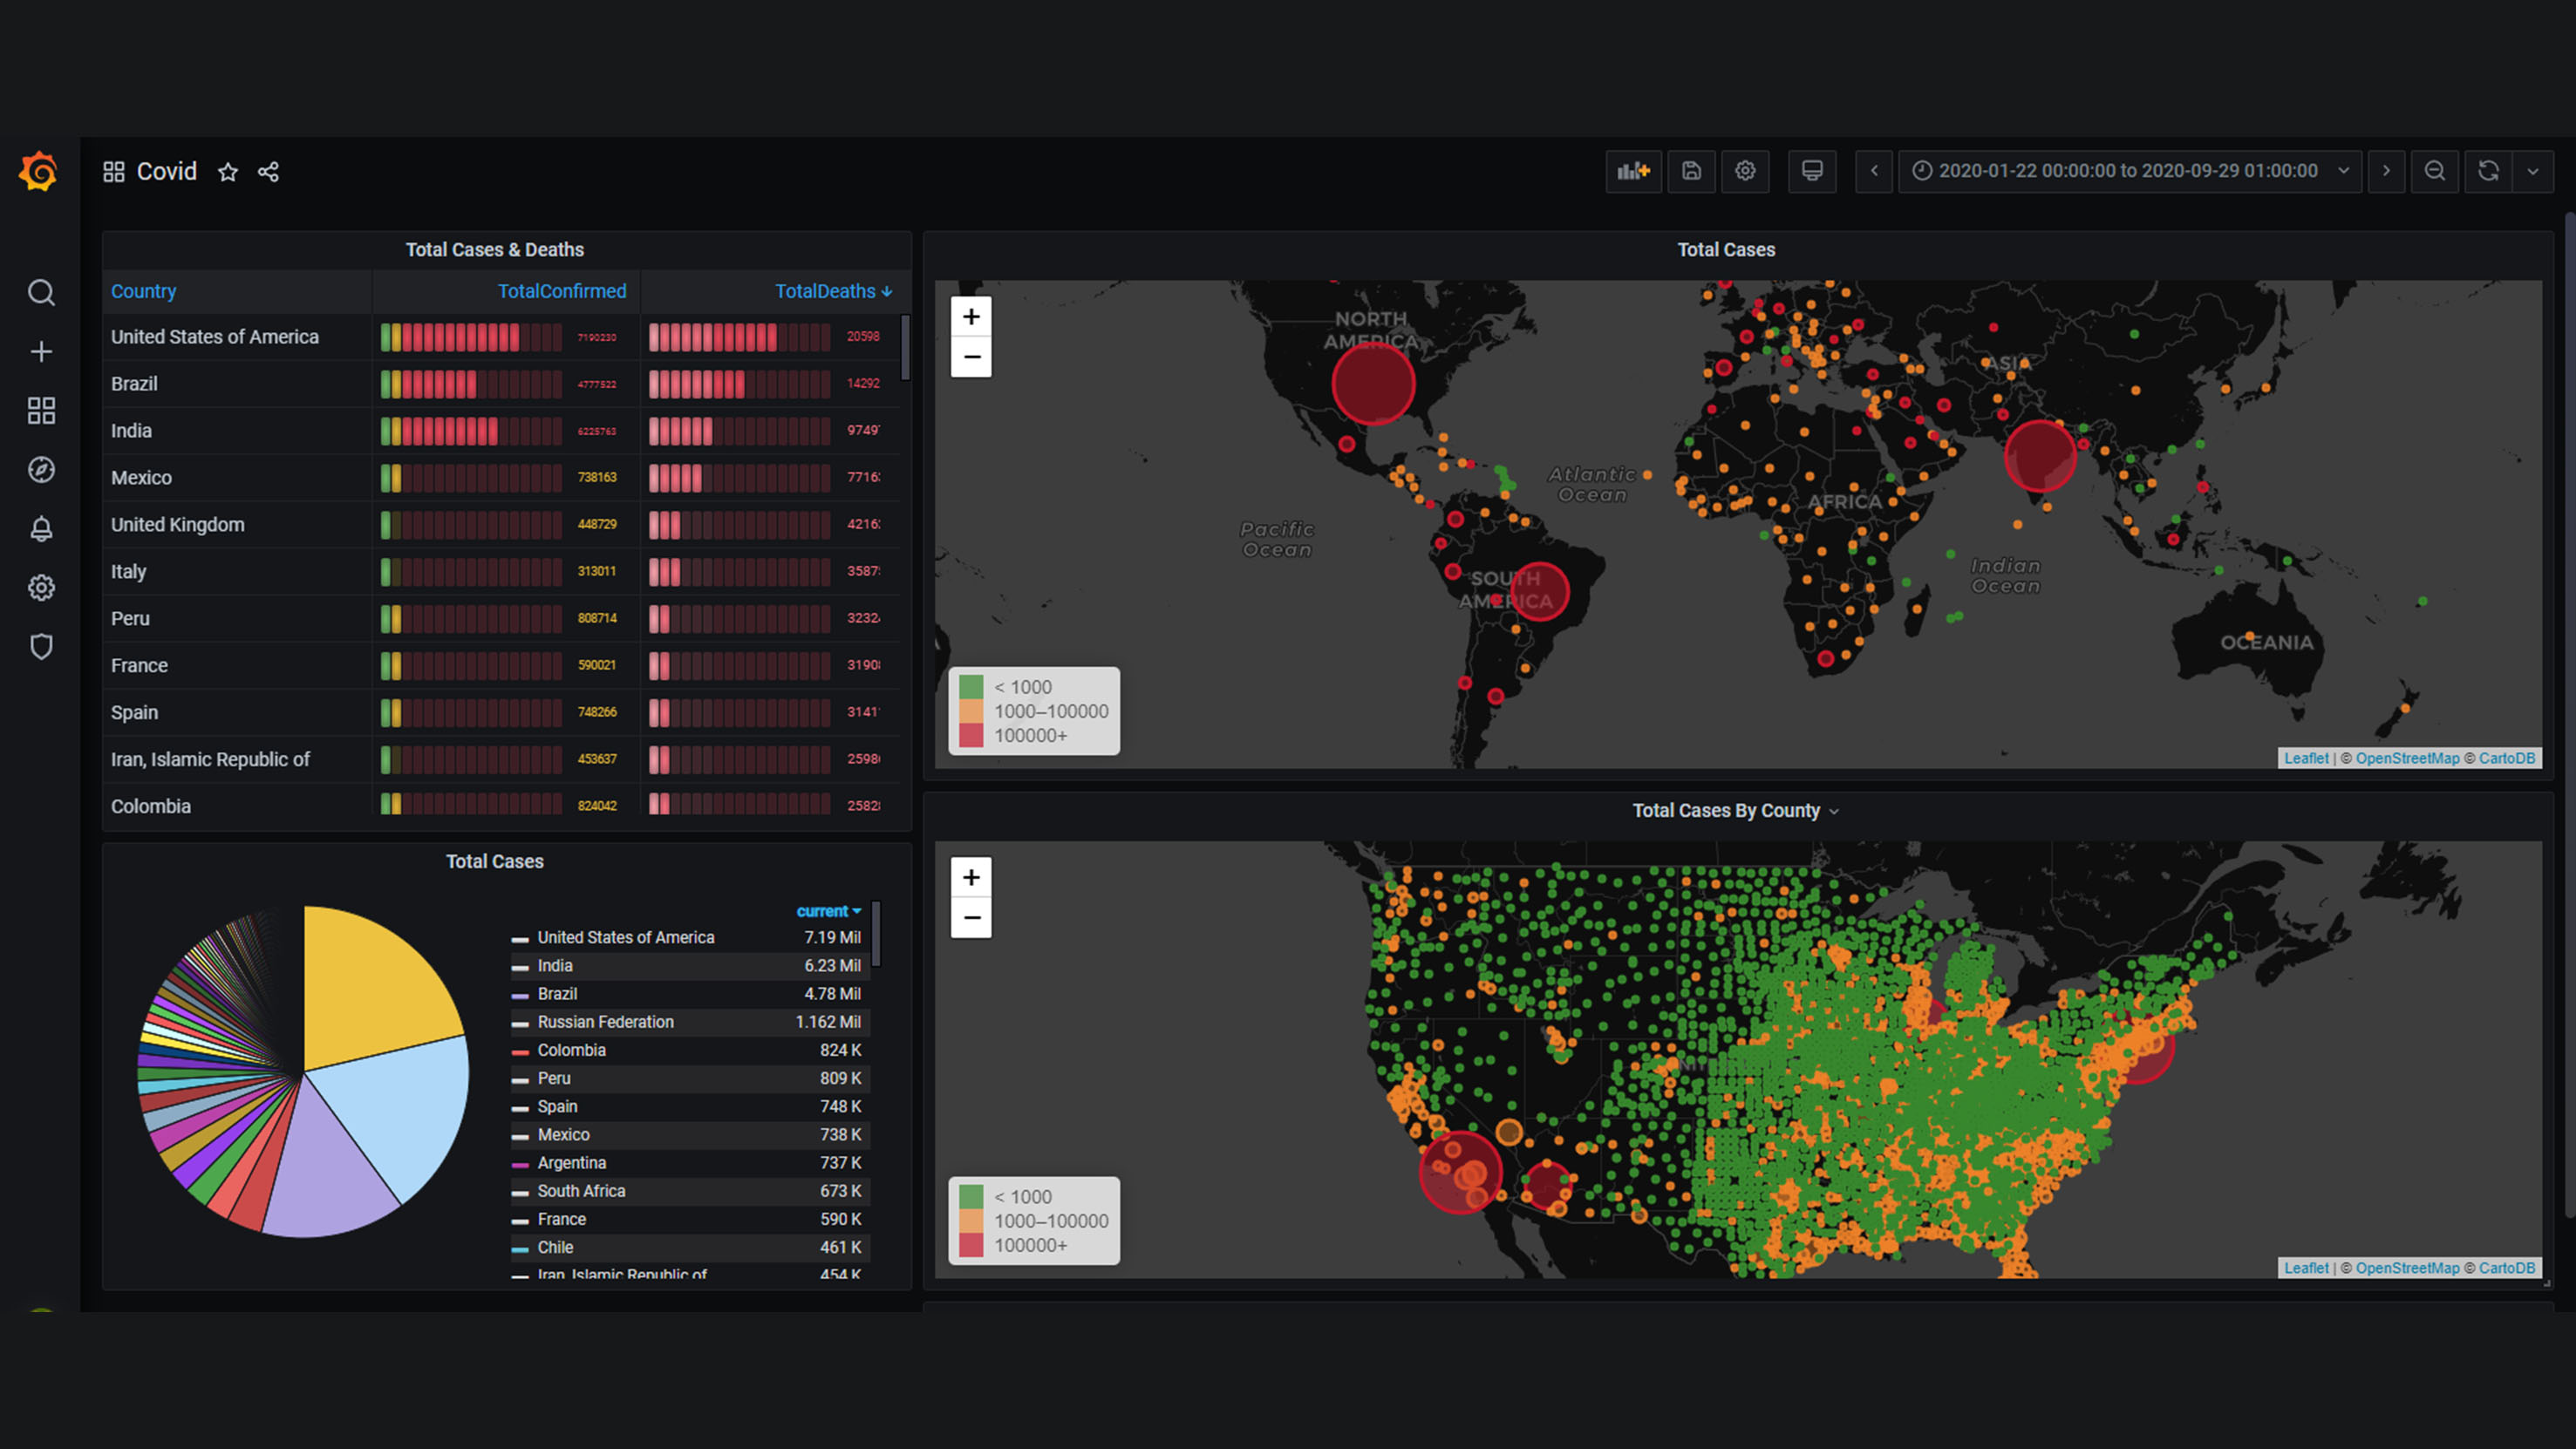
\includegraphics[width=1\textwidth]{figures/Grafana8_Covid19.jpg} 
    \caption{Dashboard theo dõi tình hình dịch bệnh Covid19} % Creates caption underneath graph
    \label{fig:fig_01}
\end{figure}
\begin{figure}[H] % places figure environment here   
    \centering % Centers Graphic
    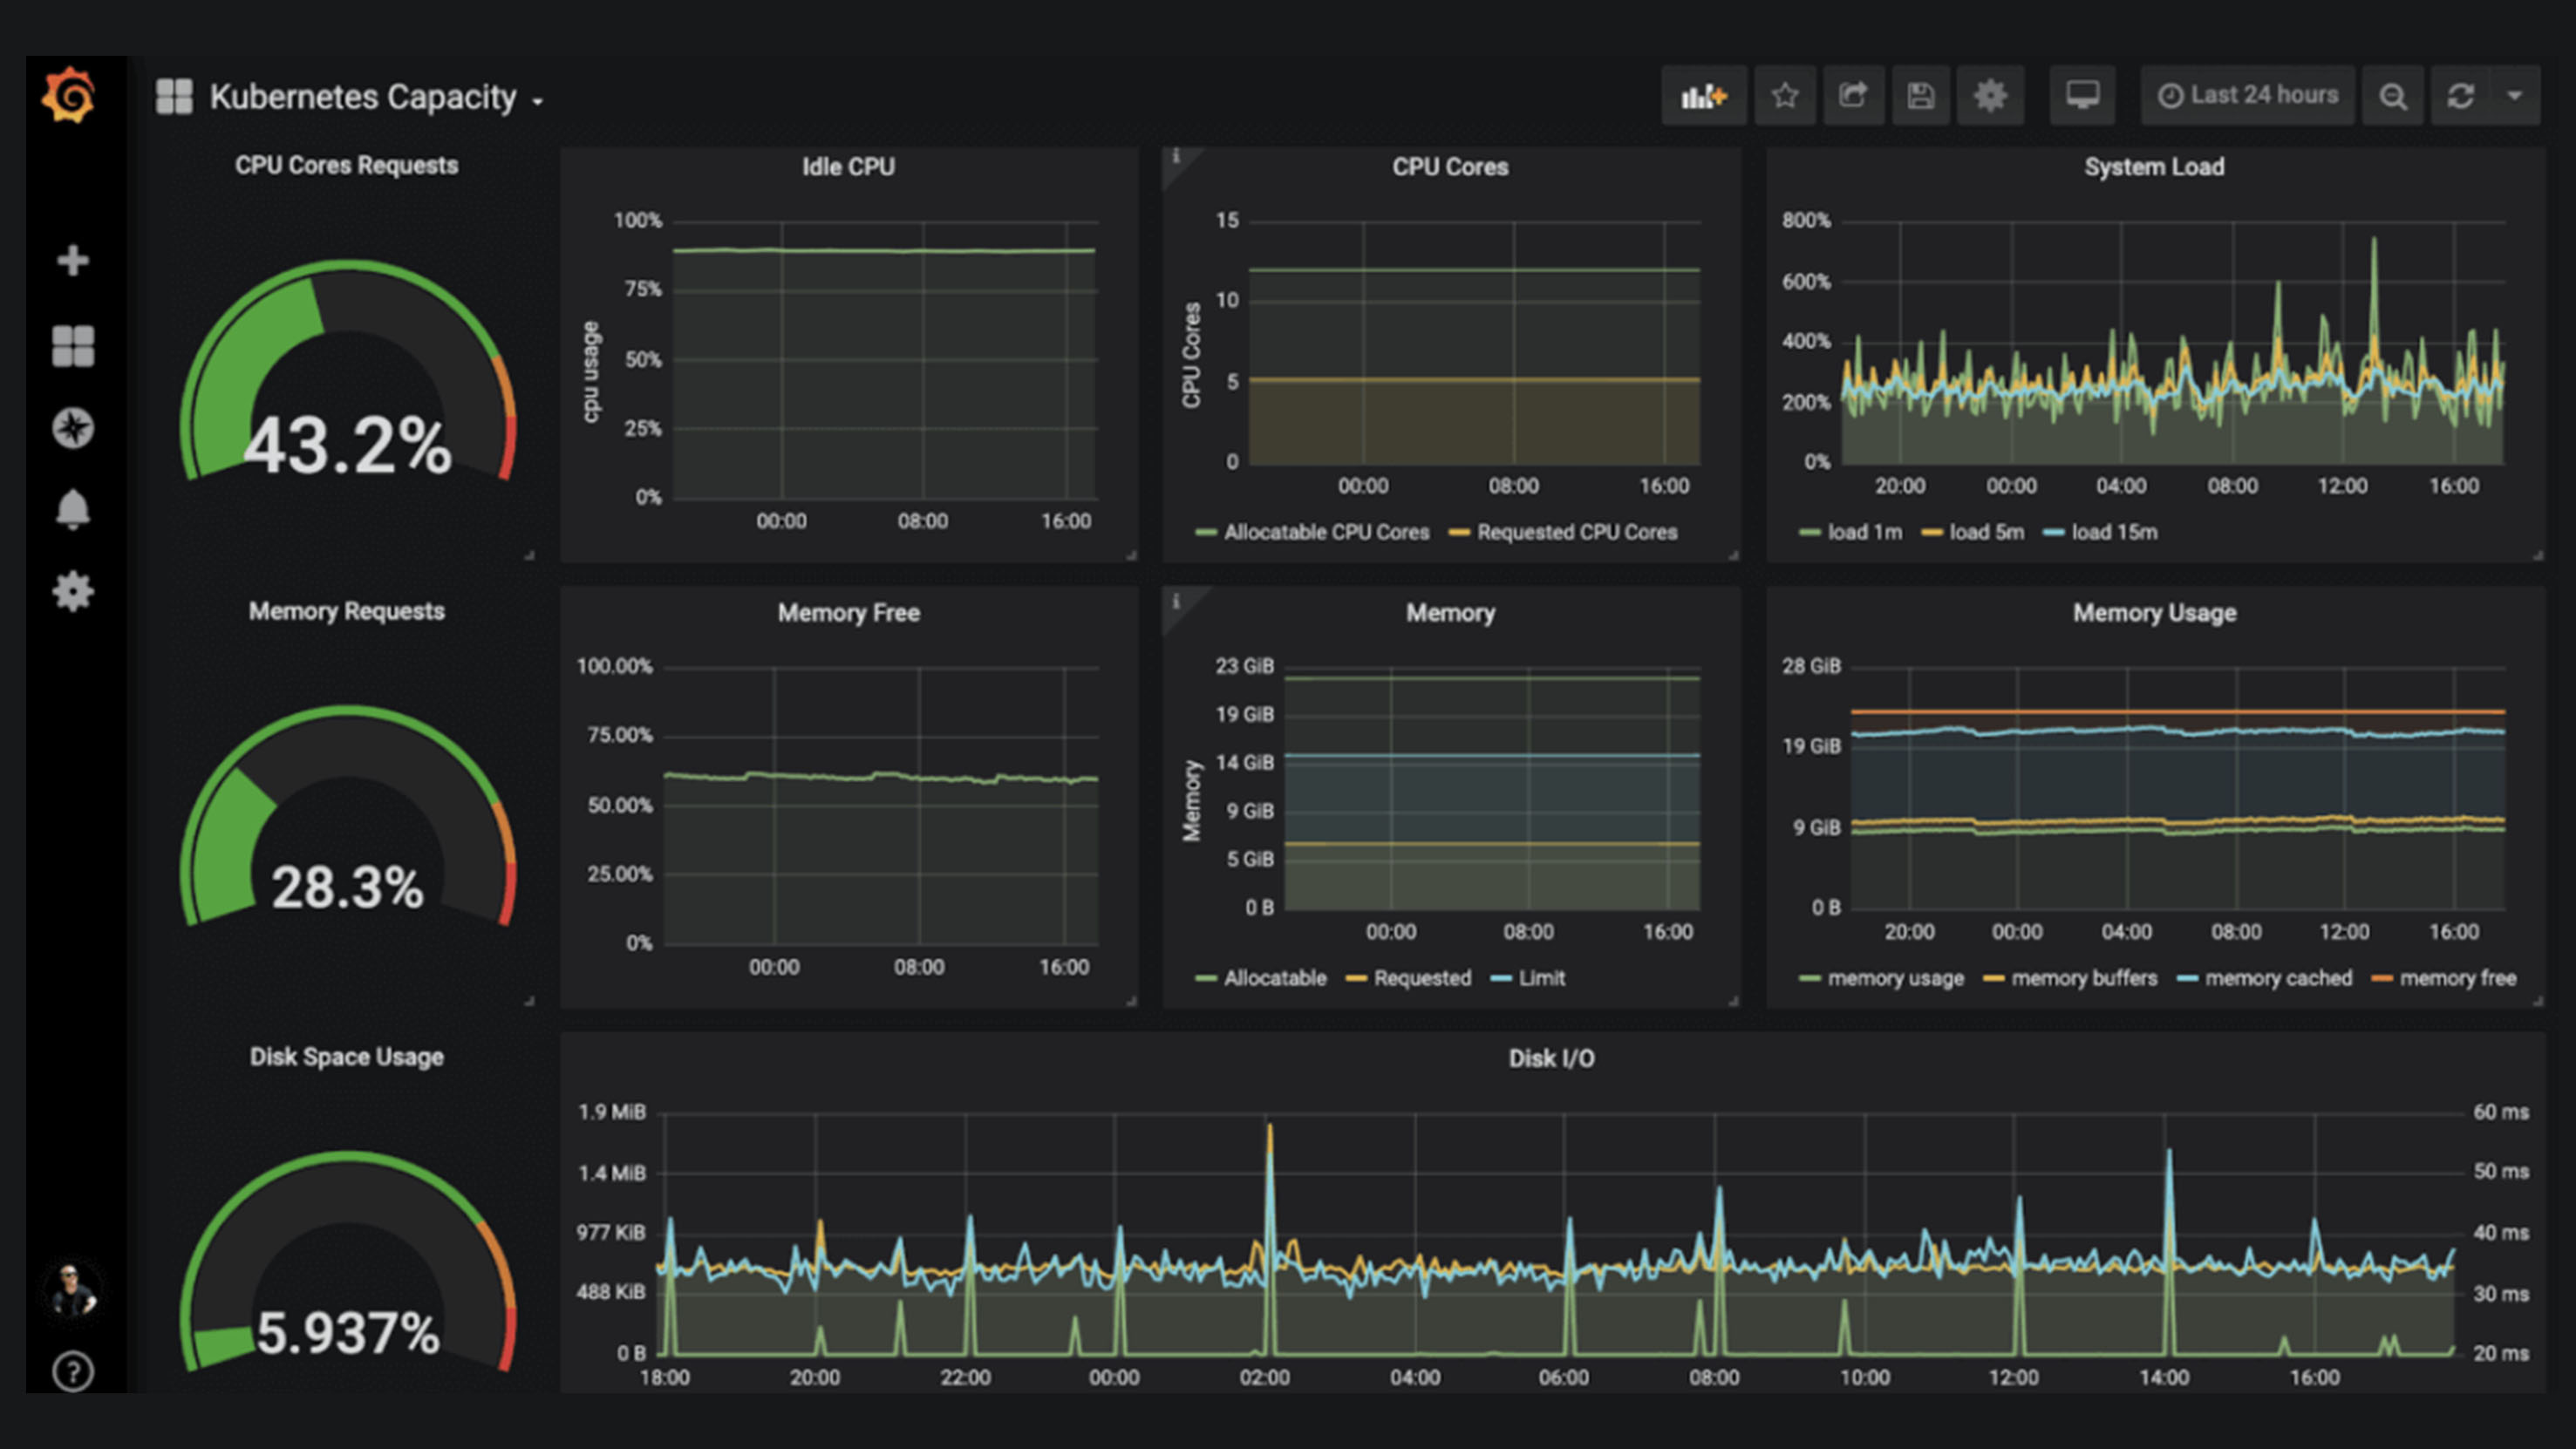
\includegraphics[width=1\textwidth]{figures/Grafana8_Kubernetes.jpg} 
    \caption{Dashboard theo dõi sức chứa hệ thống} % Creates caption underneath graph
    \label{fig:fig_01}
\end{figure}
